\section{Augmentation}
Veri artırma, veri setini çeşitlendirmek ve modelin daha genel bir anlayış geliştirmesine yardımcı olmak için mevcut verilere çeşitli yöntemler uygulayarak yeni veriler elde etme işlemidir. Bu teknik, özellikle modelin aşırı uyum (overfitting) problemiyle karşı karşıya olduğu durumlarda etkili bir çözüm sağlar. 

\subsection{Veri Türleri ve Veri Artırma Teknikleri}
\textbf{Görüntü Verileri}
\begin{itemize}
    \item \textbf{Döndürme:} Görüntüyü rastgele açılarda döndürmek.
    \item \textbf{Öteleme:} Görüntüyü yatay veya dikey olarak kaydırmak.
    \item \textbf{Kırpma:} Görüntünün rastgele parçalarını kırpmak.
    \item \textbf{Ölçeklendirme:} Görüntüyü büyütmek veya küçültmek.
    \item \textbf{Aydınlatma:} Görüntünün parlaklığını ve kontrastını değiştirmek.
    \item \textbf{Renk:} Görüntü üzerindeki renkleri değiştirmek.
\end{itemize}

\textbf{Ses Verileri}
\begin{itemize}
    \item \textbf{Gürültü ekleme:} Rastgele gürültüler ekleyerek yeni ses örneği oluşturmak.
    \item \textbf{Zaman kaydırma:} Sesi zaman ekseni boyunca kaydırmak.
    \item \textbf{Perde değiştirme:} Sesin perdesini değiştirmek.
    \item \textbf{Hız değiştirme:} Sesin hızını arttırmak veya azaltmak.
    \item \textbf{Ses sıkıştırma:} Sesi farklı sıkıştırma seviyeleriyle sıkıştırmak.
\end{itemize}

\textbf{Metin Verileri}
\begin{itemize}
    \item \textbf{Eş anlamlılarla değiştirme:} Metindeki bazı kelimeleri eş anlamlılarıyla değiştirme.
    \item \textbf{Kelime ekleme:} Metinden rastgele kelimeler eklemek.
    \item \textbf{Kelime silme:} Metinden rastgele kelimeler silmek.
    \item \textbf{Kelime sırası değiştirme:} Metindeki kelimelerin sırasını değiştirmek.
\end{itemize}

\subsection{Python ile Augmentation Teknikleri}
Gerekli kütüphaneleri yüklemekle başlayalım. Görüntü verileri için “tensorflow”, ses verileri için “librosa” ve metin verileri için “nltk” kütüphanesini kullanacağız. 

\begin{lstlisting}[language=Python]
import tensorflow as tf
import matplotlib.pyplot as plt
import numpy as np
import librosa
import random
from nltk.corpus import wordnet
from nltk.tokenize import word_tokenize
from PIL import Image
\end{lstlisting}

\subsection{Image Augmentation}
\begin{lstlisting}
# Fotograf Linki: https://unsplash.com/photos/parked-white-ford-explorer-suv-a4S6KUuLeoM 
image_path = "suv.jpg"
img = Image.open(image_path)
image = tf.io.read_file(image_path)

plt.imshow(img)
\end{lstlisting}

\begin{figure}[ht]
    \centering
    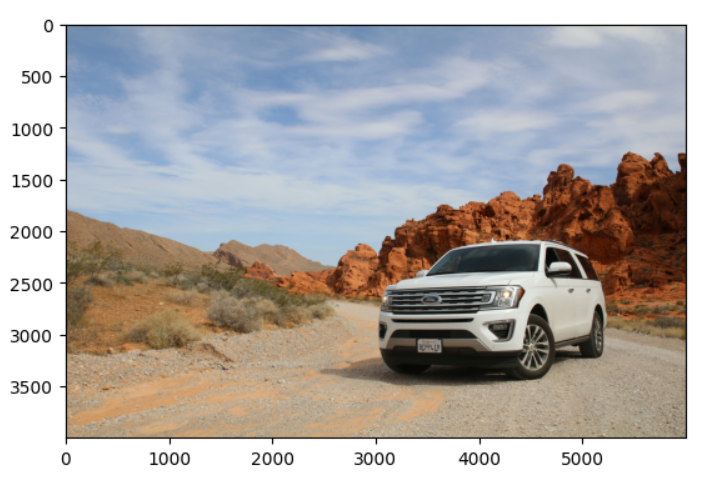
\includegraphics[width=0.5\textwidth]{images/image_aug_01.png}
    \caption{Yüklenen fotoğraf.}
    \label{fig:enter-label}
\end{figure}

\subsubsection{3 Kanallı RGB Resim Okuma}

\begin{lstlisting}[language=Python]
image_3 = tf.image.decode_jpeg(image, channels=3)

plt.imshow(image_3)
\end{lstlisting}

\newpage

\begin{figure}[ht]
    \centering
    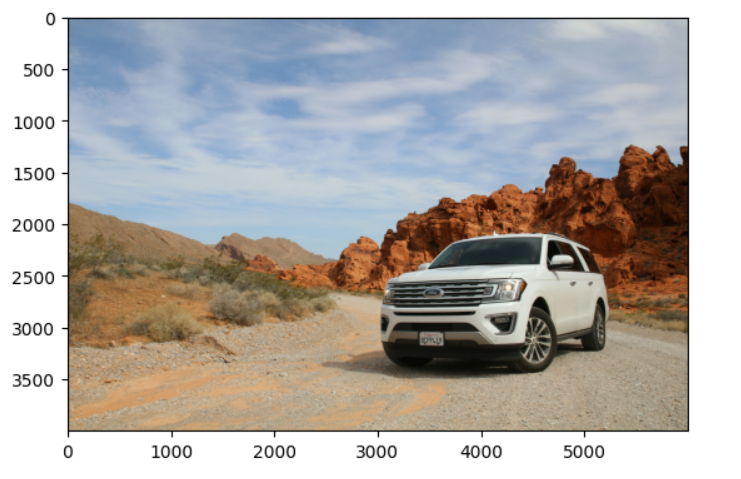
\includegraphics[width=0.5\textwidth]{images/image_aug_02.png}
    \caption{3 kanallı RGB resim okuma.}
    \label{fig:enter-label}
\end{figure}

\subsubsection{1 Kanallı Resim Okuma}

\begin{lstlisting}[language=Python]
image_1 = tf.image.decode_jpeg(image, channels=1)

plt.imshow(image_1)
\end{lstlisting}

\begin{figure}[h]
    \centering
    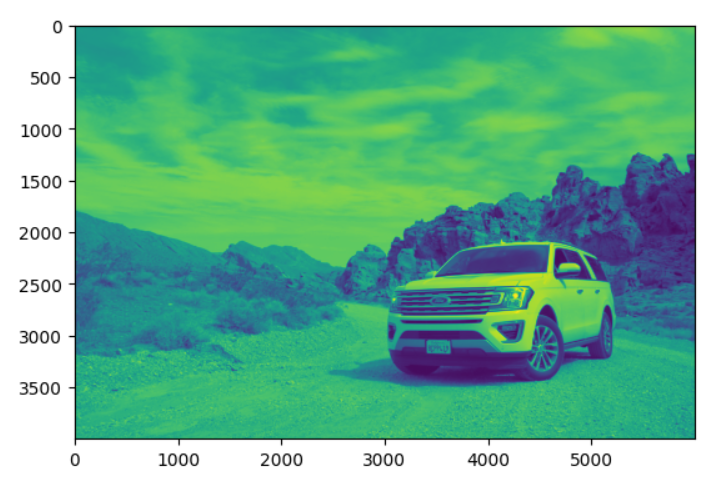
\includegraphics[width=0.5\textwidth]{images/image_aug_03.png}
    \caption{1 kanallı resim okuma.}
    \label{fig:enter-label}
\end{figure}

\subsubsection{Flip (Ters Çevirme)}

\begin{lstlisting}[language=Python]
# Goruntuyu yatay olarak ters cevirme
flipped_image = tf.image.flip_left_right(image_3)

plt.imshow(flipped_image)
\end{lstlisting}

\newpage

\begin{figure}[h]
    \centering
    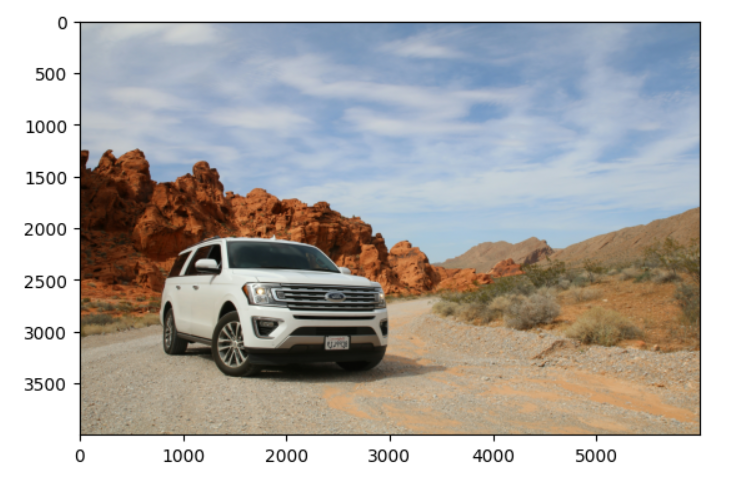
\includegraphics[width=0.5\textwidth]{images/image_aug_04.png}
    \caption{Yatay ters çevrilmiş görüntü.}
    \label{fig:enter-label}
\end{figure}

\begin{lstlisting}[language=Python]
# Goruntuyu dikey olarak ters cevirme
flipped_image = tf.image.flip_up_down(image_3)

plt.imshow(flipped_image)
\end{lstlisting}

\begin{figure}[h]
    \centering
    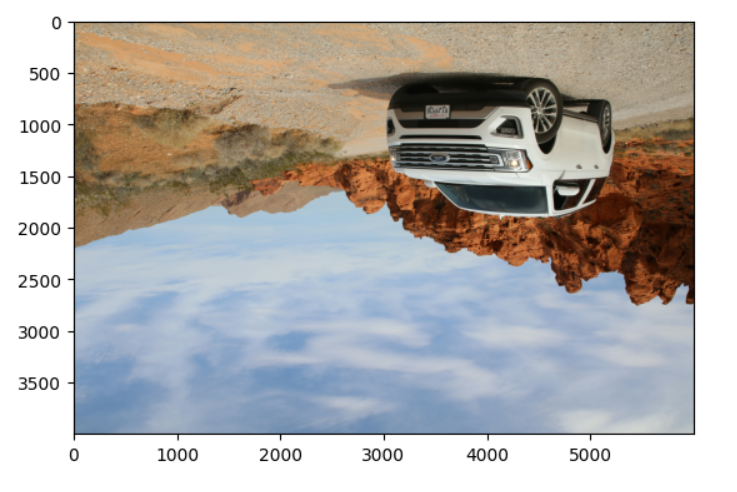
\includegraphics[width=0.5\textwidth]{images/image_aug_05.png}
    \caption{Dikey ters çevrilmiş görüntü.}
    \label{fig:enter-label}
\end{figure}

\subsubsection{Brightness (Parlaklık)}

\begin{lstlisting}[language=Python]
# Parlakligi 0.2 birim artirma
brightness_image = tf.image.adjust_brightness(image_3, delta=0.2)

plt.imshow(brightness_image)
\end{lstlisting}

\newpage

\begin{figure}[h]
    \centering
    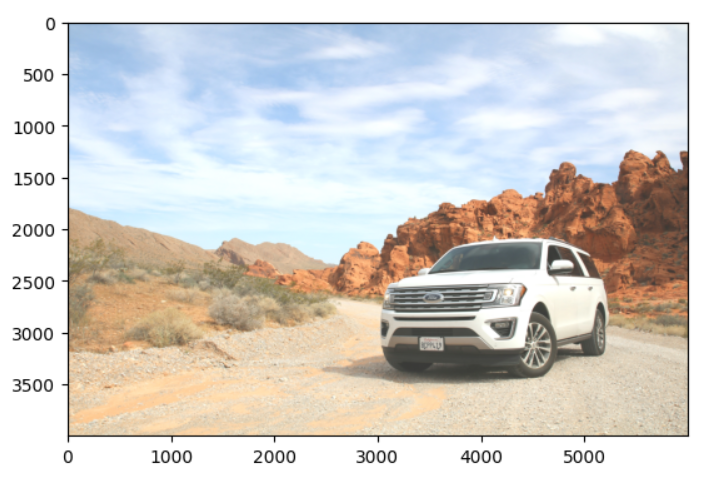
\includegraphics[width=0.5\textwidth]{images/image_aug_06.png}
    \caption{Parlaklığı 0.2 birim artırılmış görüntü.}
    \label{fig:enter-label}
\end{figure}

\subsubsection{Contrast (Kontrast)}

\begin{lstlisting}[language=Python]
# Kontrasti 2 katina cikarma
contrast_image = tf.image.adjust_contrast(image_3, contrast_factor=2)

plt.imshow(contrast_image)
\end{lstlisting}

\begin{figure}[h]
    \centering
    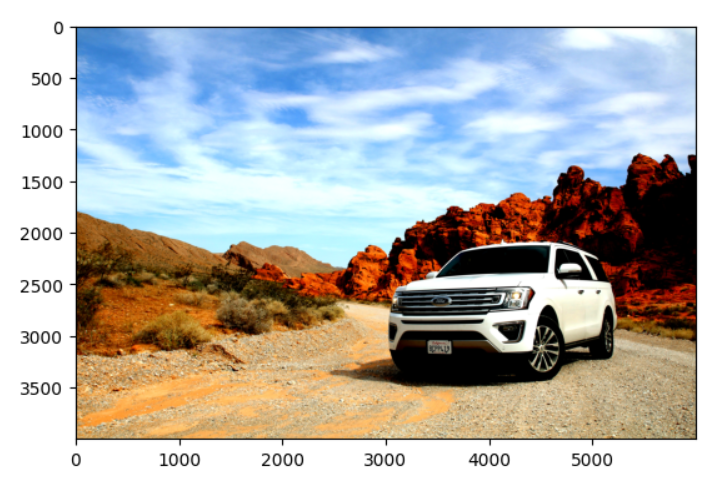
\includegraphics[width=0.5\textwidth]{images/image_aug_07.png}
    \caption{Kontrastı iki katına çıkarılmış görüntü.}
    \label{fig:enter-label}
\end{figure}

\subsubsection{Saturation (Dolgunluk)}

\begin{lstlisting}[language=Python]
#  Doygunlugu 3 katina cikarma
saturation_image = tf.image.adjust_saturation(image_3, saturation_factor=3)

plt.imshow(saturation_image)
\end{lstlisting}

\newpage

\begin{figure}[h]
    \centering
    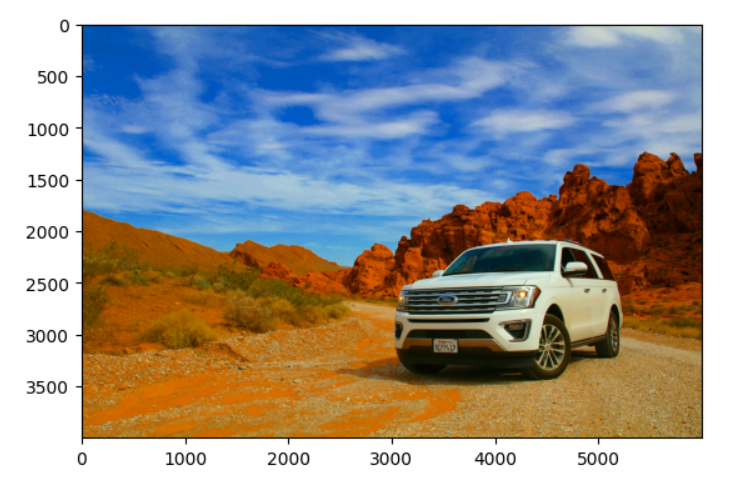
\includegraphics[width=0.5\textwidth]{images/image_aug_08.png}
    \caption{Doygunluğu üç katına çıkarılmış görüntü.}
    \label{fig:enter-label}
\end{figure}

\subsubsection{Hue (Ton)}

\begin{lstlisting}[language=Python]
# Tonu 0.1 birim degistirme
hue_image = tf.image.adjust_hue(image_3, delta=0.1)

plt.imshow(hue_image)
\end{lstlisting}

\begin{figure}[h]
    \centering
    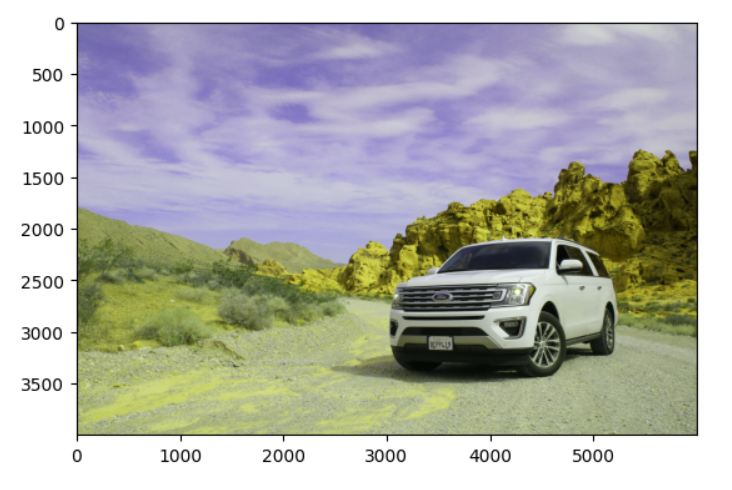
\includegraphics[width=0.5\textwidth]{images/image_aug_09.png}
    \caption{Tonu 0.1 birim değiştirilmiş görüntü.}
    \label{fig:enter-label}
\end{figure}

\subsubsection{Rotate (Döndürme)}

\begin{lstlisting}[language=Python]
# Resmi 90 derece saat yonunde dondurme.
rotated_image = tf.image.rot90(image_3)

plt.imshow(rotated_image)
\end{lstlisting}

\newpage

\begin{figure}[h]
    \centering
    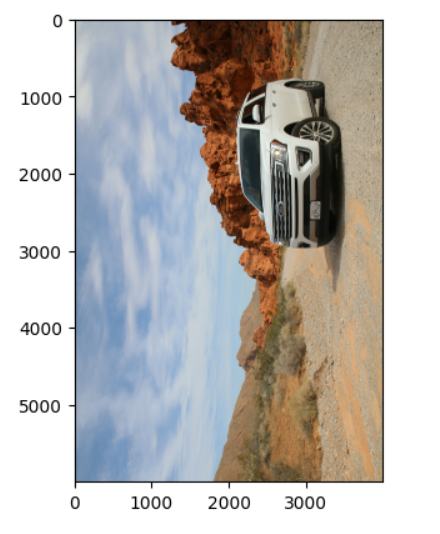
\includegraphics[width=0.5\textwidth]{images/image_aug_10.png}
    \caption{Saat yönünde 90 derece döndürülmüş görüntü.}
    \label{fig:enter-label}
\end{figure}

\subsubsection{Zoom (Yakınlaştırılma)}

\begin{lstlisting}[language=Python]
# Resmi merkezi %50 oraninda kirpma
zoomed_image = tf.image.central_crop(image_3, central_fraction=0.5)

plt.imshow(zoomed_image)
\end{lstlisting}

\begin{figure}[h]
    \centering
    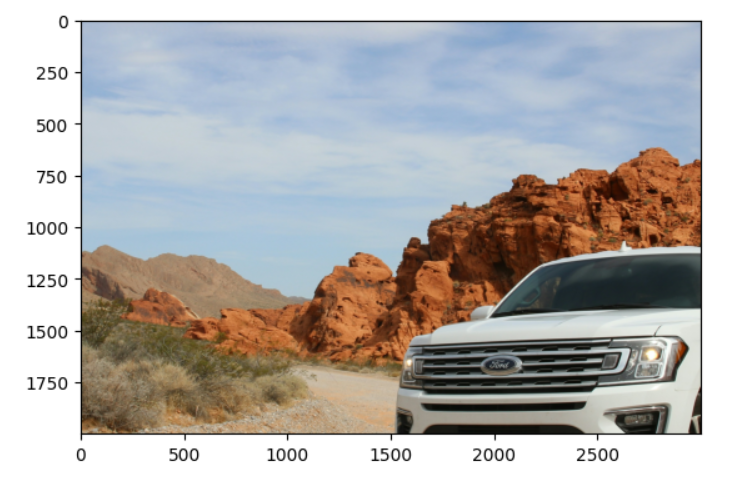
\includegraphics[width=0.5\textwidth]{images/image_aug_11.png}
    \caption{Merkezi \%50 oranında yakınlaştırılmış görüntü.}
    \label{fig:enter-label}
\end{figure}

\newpage

\subsubsection{Shear (Eğme)}

\begin{lstlisting}[language=Python]
# Resmi 45 derece egme
sheared_image = tf.keras.preprocessing.image.apply_affine_transform(image_3, shear=45)

plt.imshow(sheared_image)
\end{lstlisting}

\begin{figure}[h]
    \centering
    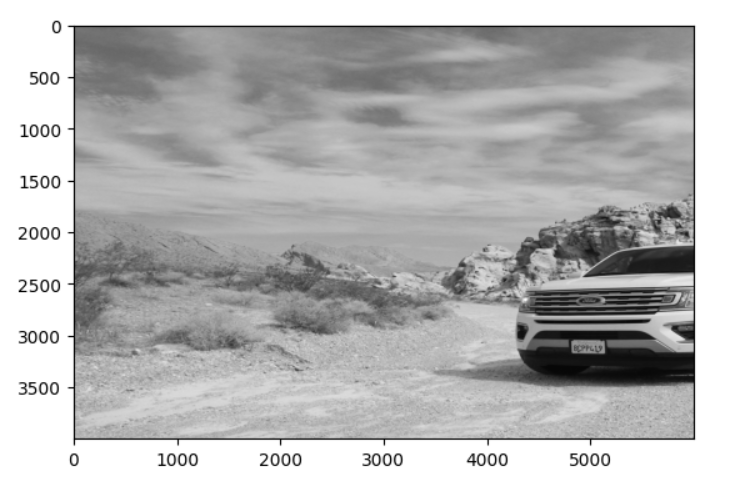
\includegraphics[width=0.5\textwidth]{images/image_aug_12.png}
    \caption{45 derece eğilmiş görüntü.}
    \label{fig:enter-label}
\end{figure}

\subsubsection{Shift (Kaydırma)}

\begin{lstlisting}[language=Python]
# Resmi 150 birim yatay ve dikey olarak kaydirma.
shifted_image = tf.keras.preprocessing.image.apply_affine_transform(image_3, tx=150, ty=150)

plt.imshow(shifted_image)
\end{lstlisting}

\begin{figure}[h]
    \centering
    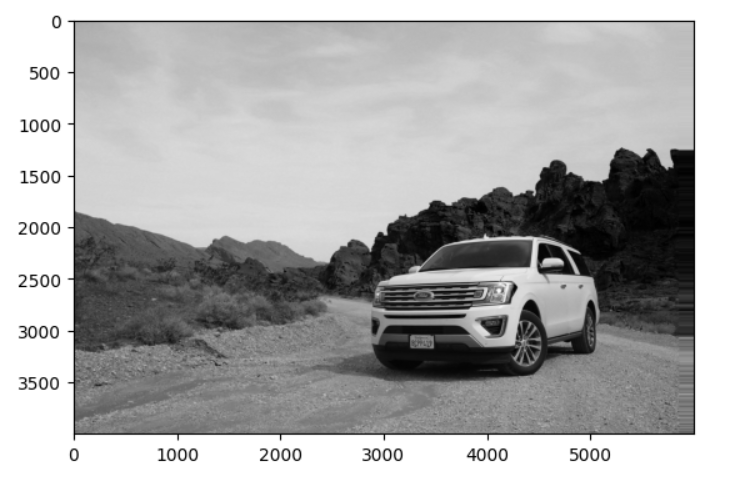
\includegraphics[width=0.5\textwidth]{images/image_aug_13.png}
    \caption{Yatay ve dikeyde 150 birim kaydırılmış  görüntü.}
    \label{fig:enter-label}
\end{figure}

\newpage

\subsection{Sound Augmentation}
Her ses dosyasında kullanacağım için bir tane görselleştirme fonksiyonu tanımlıyorum. Librosa kütüphanesi ile örnek ses dosyasını okuyorum.

\begin{lstlisting}[language=Python]
real_audio = "dog.wav"

def plot_ad(ad_path, title):
    plt.figure(figsize=(12, 4))
    plt.plot(ad_path)
    plt.title(title)
    plt.show()

real_ad, real_sr = librosa.load(real_audio)
plot_ad(real_ad, "Ham Ses Verisi")
\end{lstlisting}

\begin{figure}[h]
    \centering
    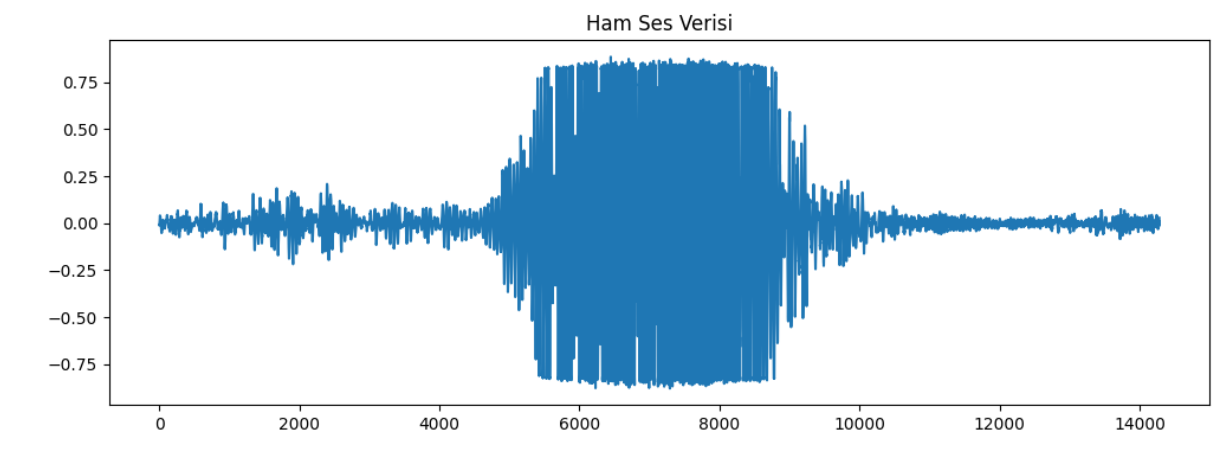
\includegraphics[width=0.7\textwidth]{images/sound_aug_01.png}
    \caption{Ham ses verisi.}
    \label{fig:enter-label}
\end{figure}

\subsubsection{Gürültü Ekleme}

\begin{lstlisting}[language=Python]
noise_factor = 0.05
noise = np.random.randn(len(real_ad))
noise_data = real_ad + noise_factor * noise

plot_ad(noise_data, "0.05 Gurultu Eklenmis Ses Verisi")
\end{lstlisting}

\begin{figure}[h]
    \centering
    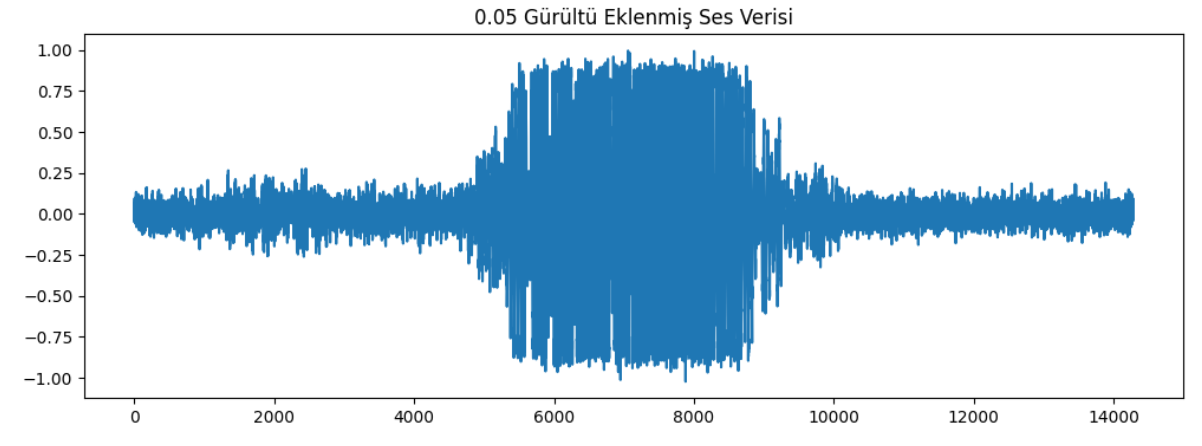
\includegraphics[width=0.7\textwidth]{images/sound_aug_02.png}
    \caption{Gürültü eklenmiş ses verisi.}
    \label{fig:enter-label}
\end{figure}

\newpage

\subsubsection{Zaman Kaydırma}

\begin{lstlisting}[language=Python]
# 0.2 saniye kaydiracagiz.
time_shift_range = int(real_sr * 0.2)
start_ = int(np.random.uniform(-time_shift_range, time_shift_range))
if start_ >= 0:
    shift_data = np.r_[real_ad[start_:], np.random.uniform(-0.001, 0.001, start_)]
else:
    shift_data = np.r_[np.random.uniform(-0.001, 0.001, -start_), real_ad[:start_]]
shift_data =  shift_data[:len(real_ad)]

plot_ad(shift_data, "0.2 Saniye Kaydirilmis Ses Verisi")
\end{lstlisting}

\begin{figure}[h]
    \centering
    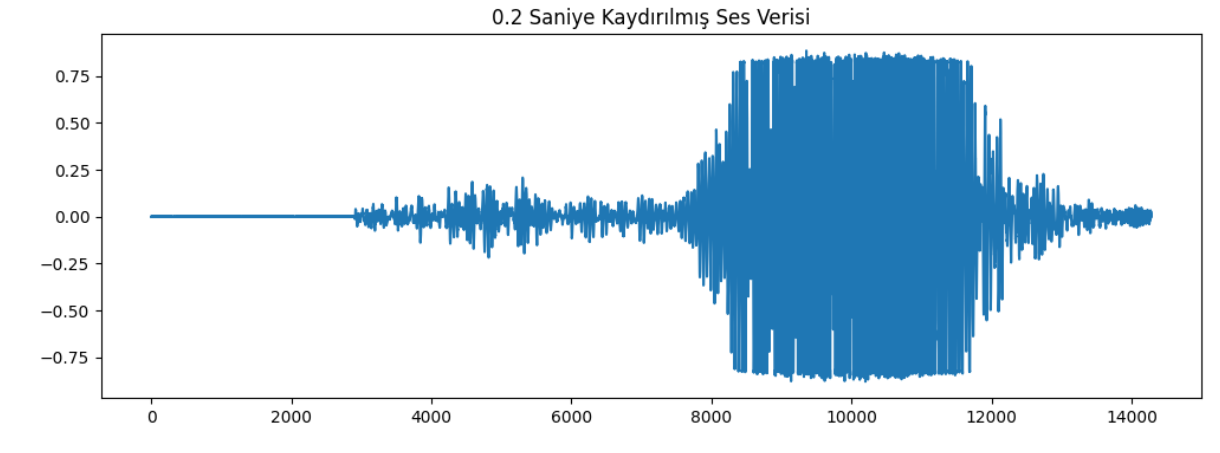
\includegraphics[width=0.7\textwidth]{images/sound_aug_03.png}
    \caption{0.2 Saniye kaydırılmış ses verisi.}
    \label{fig:enter-label}
\end{figure}

\subsubsection{Hız Değiştirme}

\begin{lstlisting}[language=Python]
speed_factor = 2
speed_data = librosa.effects.time_stretch(y=real_ad, rate=speed_factor)

plot_ad(speed_data, "2x Hizlandirilmis Ses Verisi")
\end{lstlisting}

\begin{figure}[h]
    \centering
    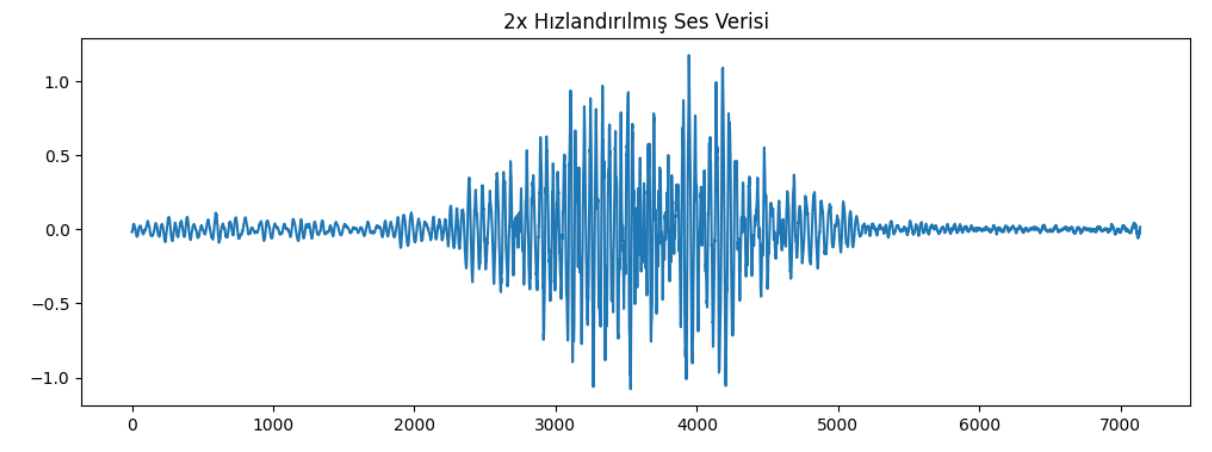
\includegraphics[width=0.7\textwidth]{images/sound_aug_04.png}
    \caption{2x Hızlandırılmış ses verisi.}
    \label{fig:enter-label}
\end{figure}

\newpage

\subsubsection{Perde Değiştirme}

\begin{lstlisting}[language=Python]
pitch_shift_factor = 1.5
pitch_data = librosa.effects.pitch_shift(y=real_ad, sr=real_sr, n_steps=pitch_shift_factor)

plot_ad(pitch_data, "1.5 Perde Degistirilmis Ses Verisi")
\end{lstlisting}

\begin{figure}[h]
    \centering
    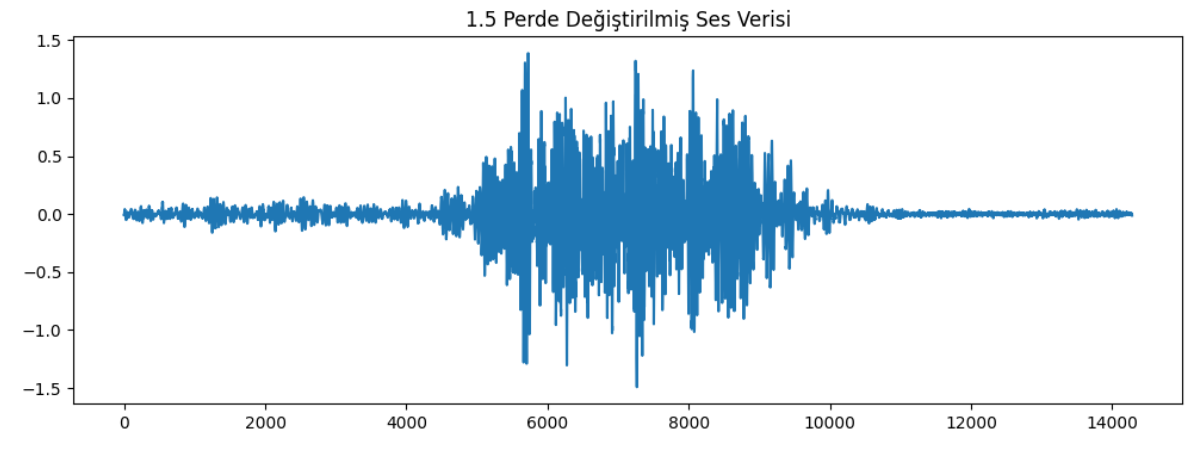
\includegraphics[width=0.7\textwidth]{images/sound_aug_05.png}
    \caption{1.5 Perde değiştirilmiş ses verisi.}
    \label{fig:enter-label}
\end{figure}

\subsection{Text Augmentation}
Örnek bir metin tanımlayıp bunun üzerinden yeni metinler elde etmeye çalışacağız.

\subsubsection{Eş Anlamlılarla Değiştirme}

\begin{lstlisting}[language=Python]
words = word_tokenize(text)
new_words = words.copy()
for i, word in enumerate(words):
    syns = wordnet.synsets(word)
    if syns:
        synonym = random.choice(syns).lemma_names()[0]
        new_words[i] = synonym

new_words = ' '.join(new_words)
print("Ham Metin:", text)
print("Es Anlamlilarla Degistirilmis Metin:", new_words)
\end{lstlisting}

\begin{figure}[h]
    \centering
    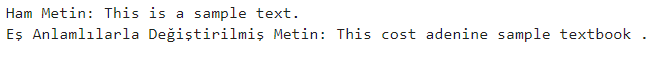
\includegraphics[width=1\textwidth]{images/text_aug_01.png}
    \caption{Eş anlamlılarla değiştirilmiş metin.}
    \label{fig:enter-label}
\end{figure}

\newpage

\subsubsection{Kelime Ekleme}

\begin{lstlisting}[language=Python]
words = word_tokenize(text)
new_words = words.copy()
random_index = random.randint(0, len(words) - 1)
new_words.insert(random_index, 'word')
new_words = ' '.join(new_words)

print("Ham Metin:", text)
print("Kelime Eklenmis Metin:", new_words)
\end{lstlisting}

\begin{figure}[h]
    \centering
    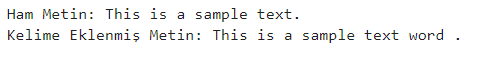
\includegraphics[width=1\textwidth]{images/text_aug_02.png}
    \caption{Kelime eklenmiş metin.}
    \label{fig:enter-label}
\end{figure}

\subsubsection{Kelime Silme}

\begin{lstlisting}[language=Python]
words = word_tokenize(text)
random_index = random.randint(0, len(words) - 1)
new_words = words[:random_index] + words[random_index + 1:]
new_words = ' '.join(new_words)

print("Ham Metin:", text)
print("Kelime Silinmis Metin:", new_words)
\end{lstlisting}

\begin{figure}[h]
    \centering
    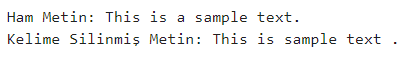
\includegraphics[width=1\textwidth]{images/text_aug_03.png}
    \caption{Kelime silinmiş metin.}
    \label{fig:enter-label}
\end{figure}

\newpage

\subsubsection{Kelime Sırası Değiştirme}

\begin{lstlisting}[language=Python]
words = word_tokenize(text)
random.shuffle(words)
new_words = ' '.join(words)

print("Ham Metin:", text)
print("Kelime Sirasi Degistirilmis Metin:", new_words)
\end{lstlisting}

\begin{figure}[h]
    \centering
    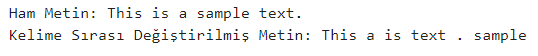
\includegraphics[width=1\textwidth]{images/text_aug_04.png}
    \caption{Kelime sırası değiştirilmiş metin.}
    \label{fig:enter-label}
\end{figure}

\newpage